\chapter{Comparação Numérica com FastBEM}

Os gráficos a seguir mostram os resultados numéricos calculados utilizando a nossa abordagem (GPU) e a abordagem anterior (FastBEM). Cada gráfico mostra a módulo dos coeficientes multipolares calculados por ambos os métodos e também a diferença numérica entre os resultados.
\begin{figure}[ht]
\centering%
\begin{subfigure}{0.45\textwidth}
	\centering
	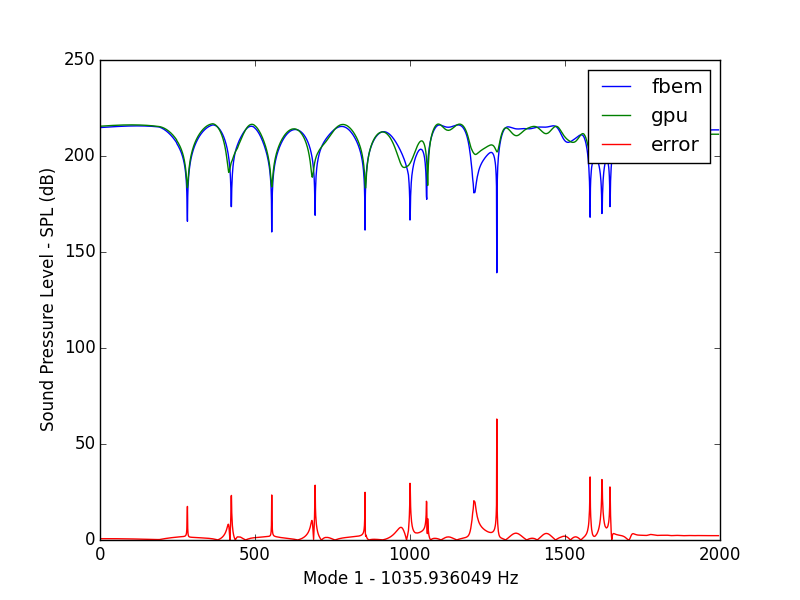
\includegraphics[width=\textwidth]{../data/transfer_test/ceramic_plate/plots/ceramic_plate-tfv-0_1.png}
	\caption{}
	\label{fig:coef_plate_1}
\end{subfigure}%
\begin{subfigure}{0.45\textwidth}
	\centering
	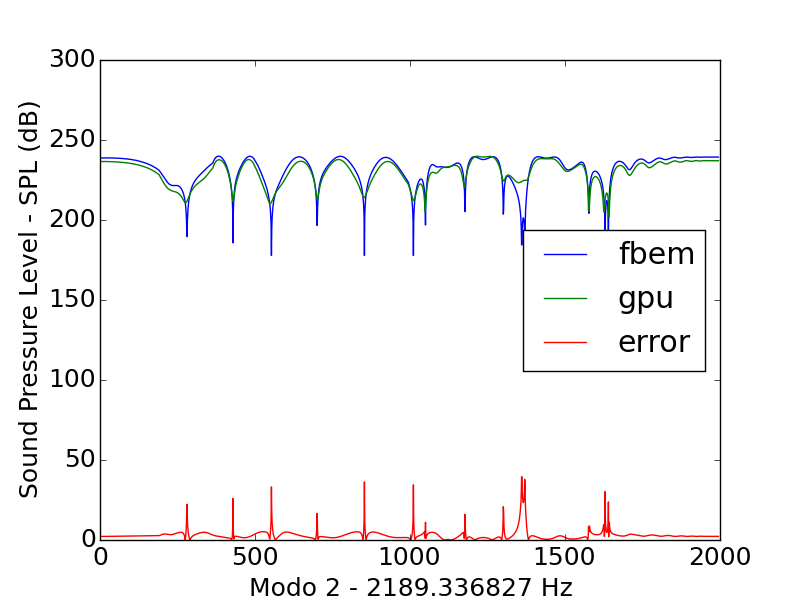
\includegraphics[width=\textwidth]{../data/transfer_test/ceramic_plate/plots/ceramic_plate-tfv-0_2.png}
	\label{fig:coef_plate_2}
	\caption{}
\end{subfigure}
\begin{subfigure}{0.45\textwidth}
	\centering
	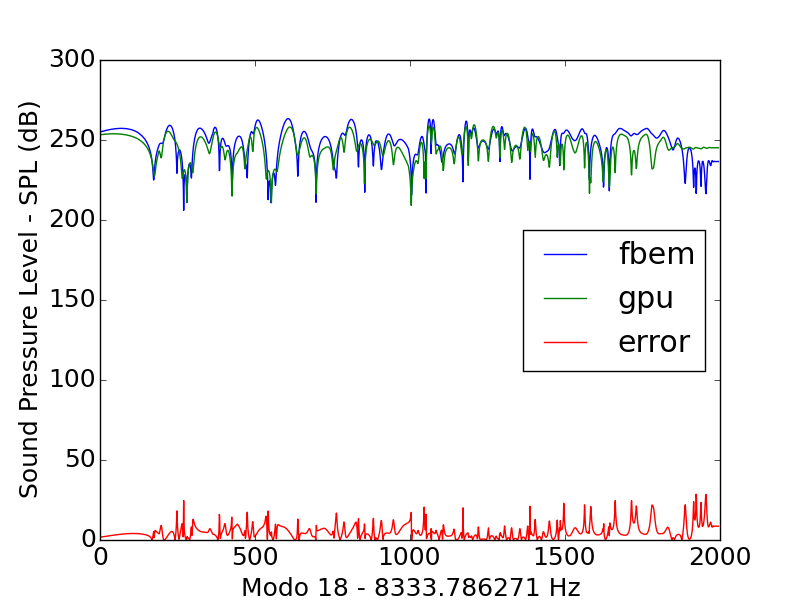
\includegraphics[width=\textwidth]{../data/transfer_test/ceramic_plate/plots/ceramic_plate-tfv-0_18.png}
	\caption{}
	\label{fig:coef_plate_18}
\end{subfigure}%
\begin{subfigure}{0.45\textwidth}
	\centering
	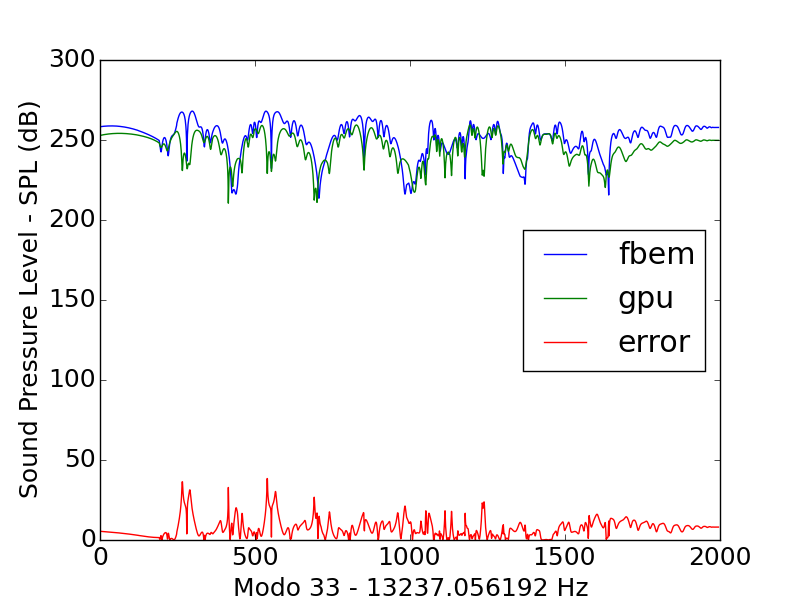
\includegraphics[width=\textwidth]{../data/transfer_test/ceramic_plate/plots/ceramic_plate-tfv-0_33.png}
	\caption{}
	\label{fig:coef_plate_33}
\end{subfigure}
\caption[Comparação numérica para o Prato de Cerâmica]{Comparação numérica para o Prato de Cerâmica. As figuras apresentam a comparação do módulo dos coeficientes para modos de vibração específicos.}
\label{fig:coef_plate}
\end{figure}

% \begin{figure}[ht] \label{fig:coef_mug_delta}
% \centering
% 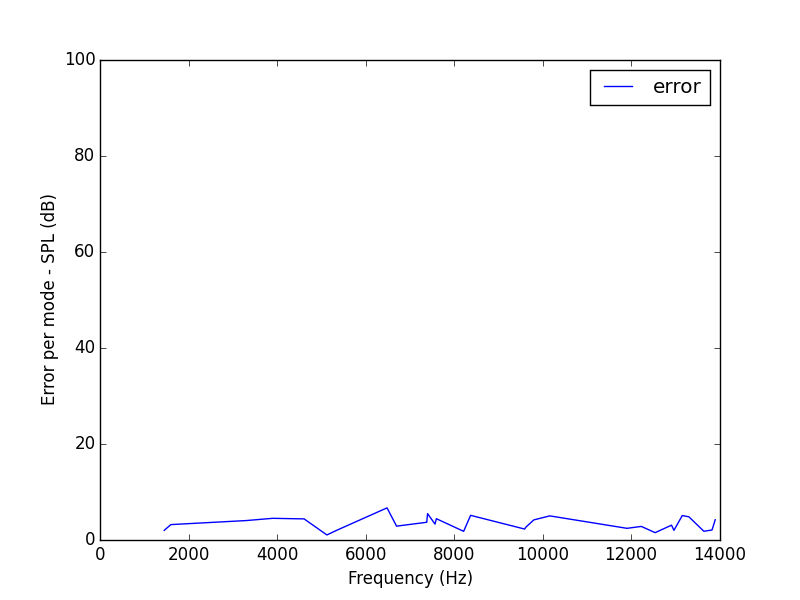
\includegraphics[width=0.6\textwidth]{../data/transfer_test/ceramic_mug/plots/ceramic_mug_error.png}
% \caption[Comparação numérica para a Caneca de Cerâmica]{Comparação numérica para a Caneca de Cerâmica. A figura ao topo apresenta o Erro Médio por frequência. As demais figuras apresentam a comparação para modos de vibração específicos.}
% \end{figure}

% \begin{figure}[ht] \label{fig:coef_key_delta}
% \centering
% 	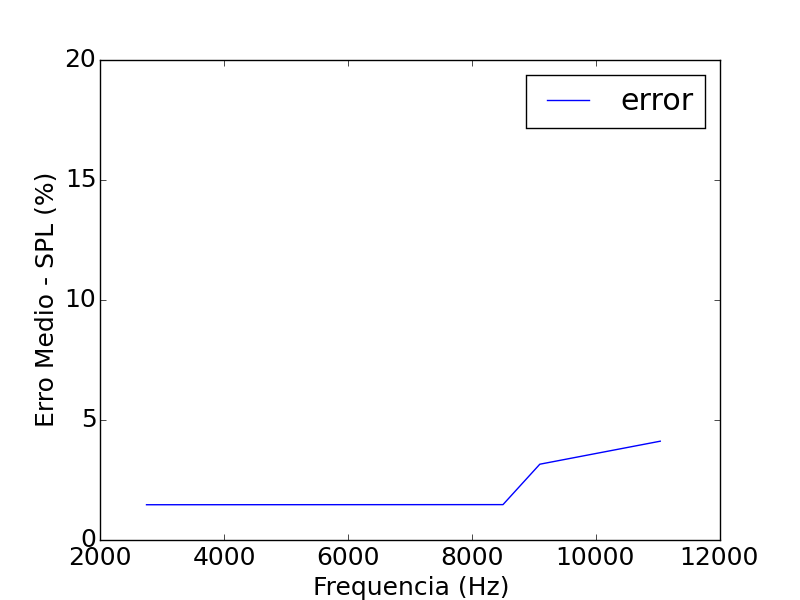
\includegraphics[width=0.6\textwidth]{../data/transfer_test/steel_key/plots/steel_key_error.png}
% \caption[Comparação numérica para a Chave de Aço]{Comparação numérica para a Chave de Aço. A figura ao topo apresenta o Erro Médio por frequência. As demais figuras apresentam a comparação para modos de vibração específicos.}
% \end{figure}

\begin{figure}[ht]
\centering
\begin{subfigure}{0.6\textwidth}
\centering
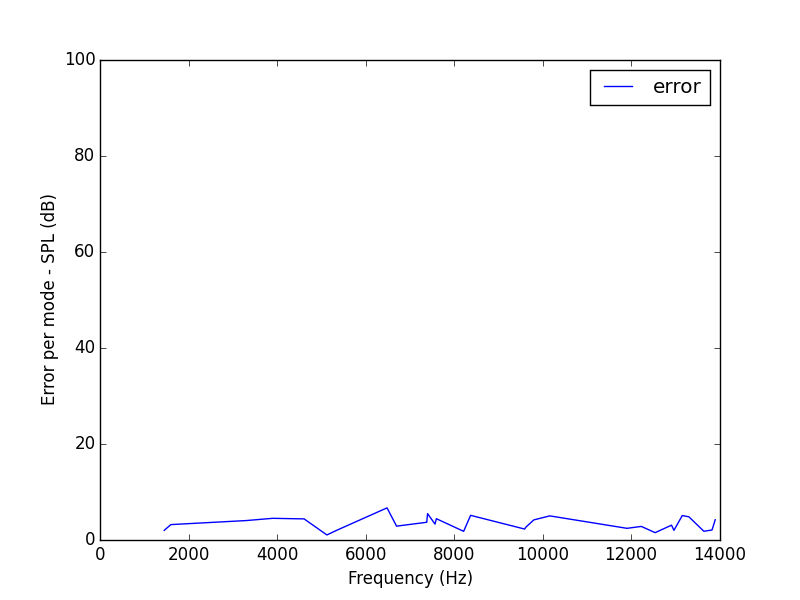
\includegraphics[width=\textwidth]{../data/transfer_test/ceramic_mug/plots/ceramic_mug_error.png}
\end{subfigure}
\begin{subfigure}{0.45\textwidth}
	\centering
	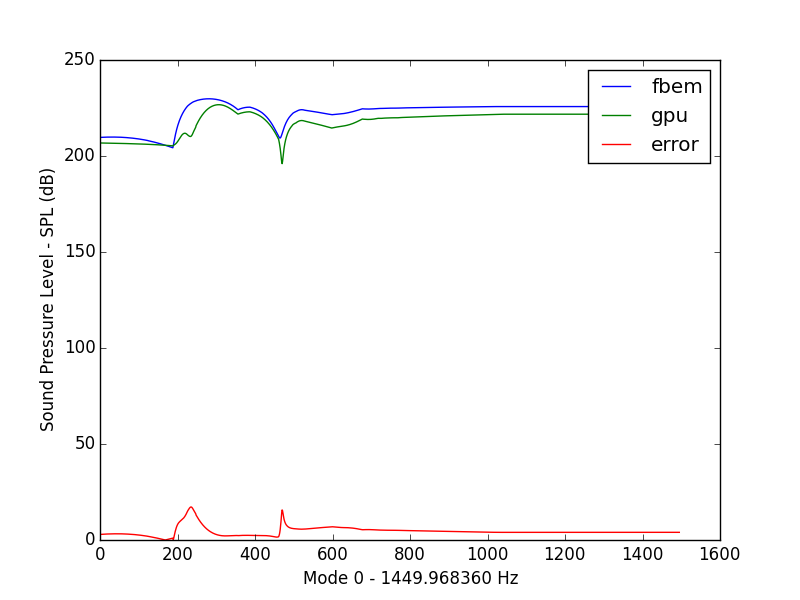
\includegraphics[width=\textwidth]{../data/transfer_test/ceramic_mug/plots/ceramic_mug-tfv-0_0.png}
	\caption{}
	\label{fig:coef_mug_0}
\end{subfigure}%
\begin{subfigure}{0.45\textwidth}
	\centering
	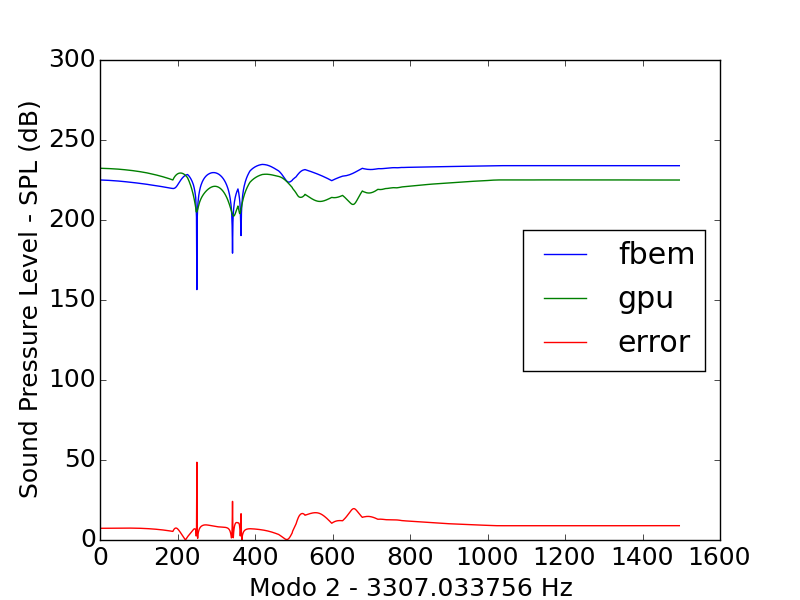
\includegraphics[width=\textwidth]{../data/transfer_test/ceramic_mug/plots/ceramic_mug-tfv-0_2.png}
	\caption{}
	\label{fig:coef_mug_2}
\end{subfigure}
\begin{subfigure}{0.45\textwidth}
	\centering
	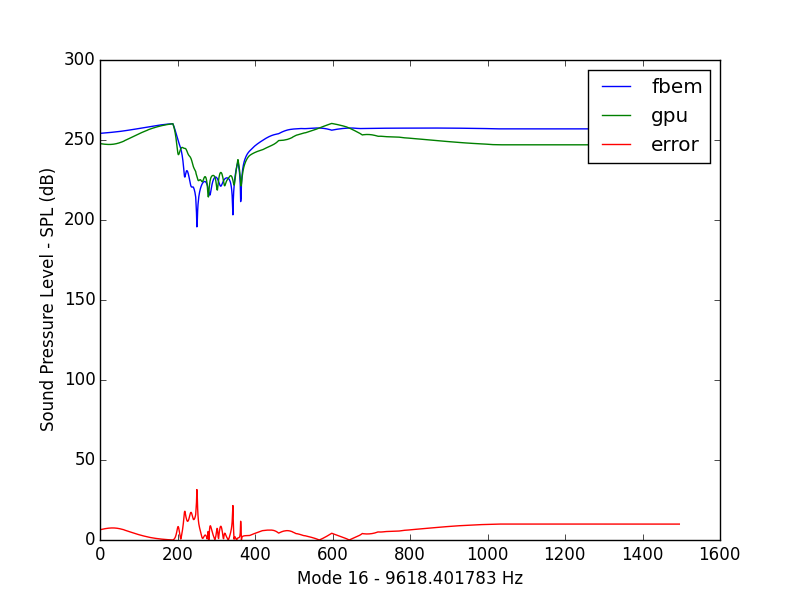
\includegraphics[width=\textwidth]{../data/transfer_test/ceramic_mug/plots/ceramic_mug-tfv-0_16.png}
	\caption{}
	\label{fig:coef_mug_16}
\end{subfigure}%
\begin{subfigure}{0.45\textwidth}
	\centering
	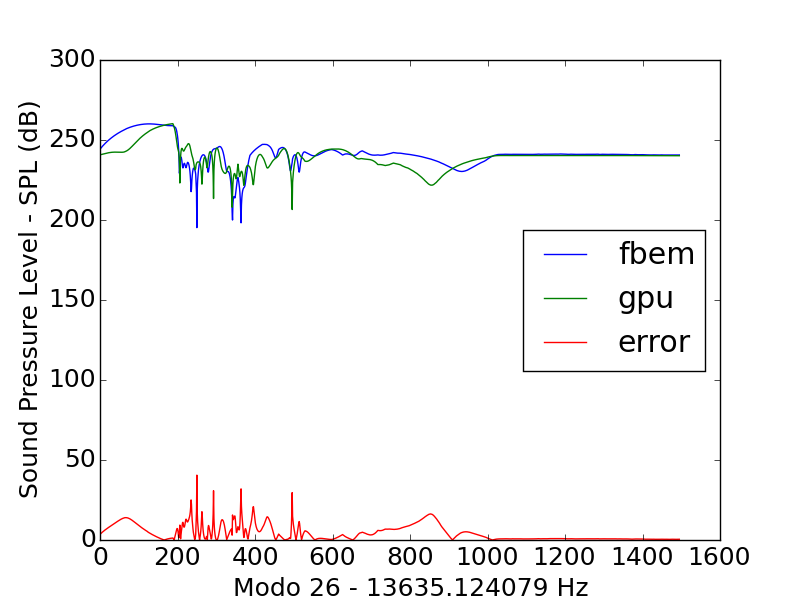
\includegraphics[width=\textwidth]{../data/transfer_test/ceramic_mug/plots/ceramic_mug-tfv-0_26.png}
	\caption{}
	\label{fig:coef_mug_26}
\end{subfigure}
\caption[Comparação numérica para a Caneca de Cerâmica]{Comparação numérica para a Caneca de Cerâmica. A figura ao topo apresenta a diferença numérica média por frequência. As demais figuras apresentam a comparação do módulo dos coeficientes para modos de vibração específicos.}
\label{fig:coef_mug_diff}
\end{figure}

\begin{figure}[ht]
\centering
\begin{subfigure}{0.6\textwidth}
\centering
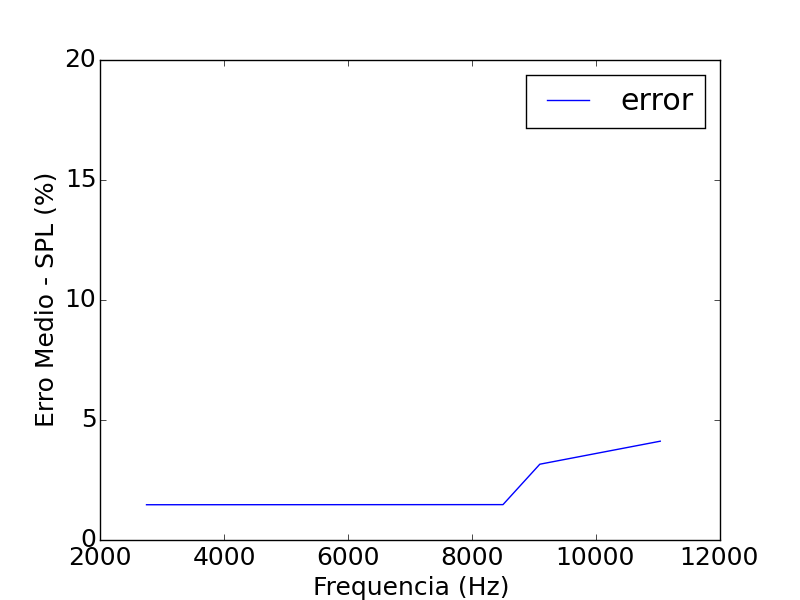
\includegraphics[width=\textwidth]{../data/transfer_test/steel_key/plots/steel_key_error.png}
\end{subfigure}
\begin{subfigure}{0.45\textwidth}
	\centering
	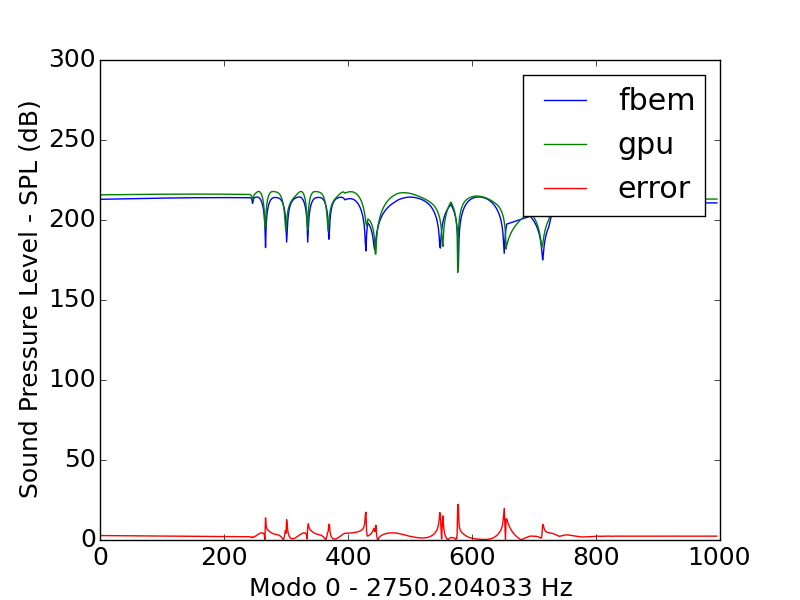
\includegraphics[width=\textwidth]{../data/transfer_test/steel_key/plots/steel_key-tfv-0_0.png}
	\caption{}
	\label{fig:coef_key_0}
\end{subfigure}%
\begin{subfigure}{0.45\textwidth}
	\centering
	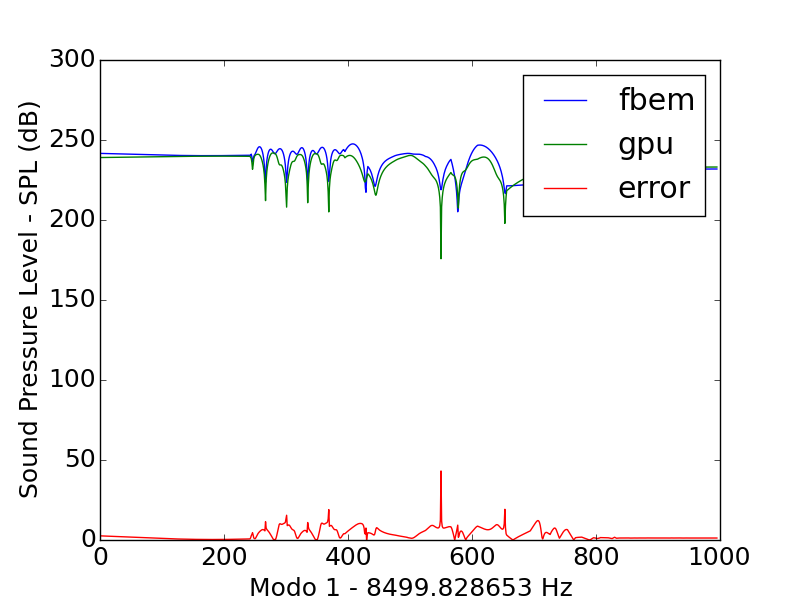
\includegraphics[width=\textwidth]{../data/transfer_test/steel_key/plots/steel_key-tfv-0_1.png}
	\caption{}
	\label{fig:coef_key_1}
\end{subfigure}
\begin{subfigure}{0.45\textwidth}
	\centering
	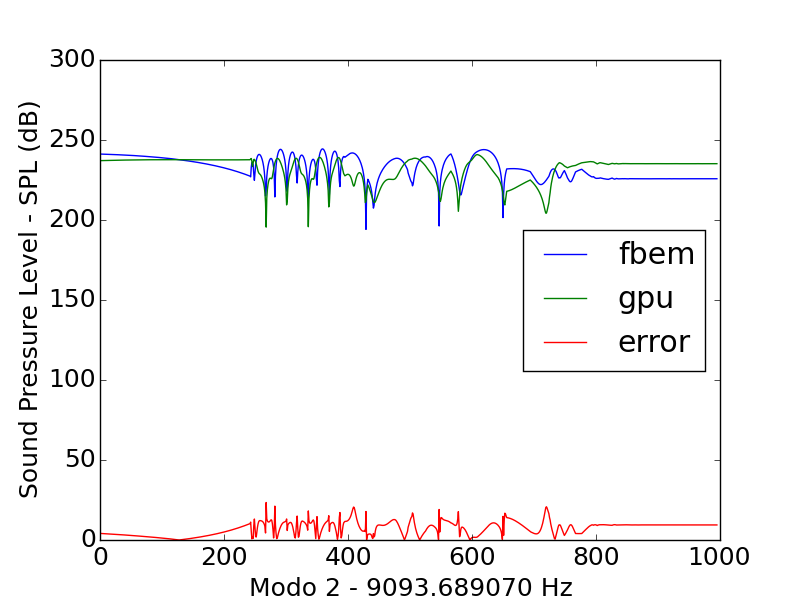
\includegraphics[width=\textwidth]{../data/transfer_test/steel_key/plots/steel_key-tfv-0_2.png}
	\caption{}
	\label{fig:coef_key_2}
\end{subfigure}%
\begin{subfigure}{0.45\textwidth}
	\centering
	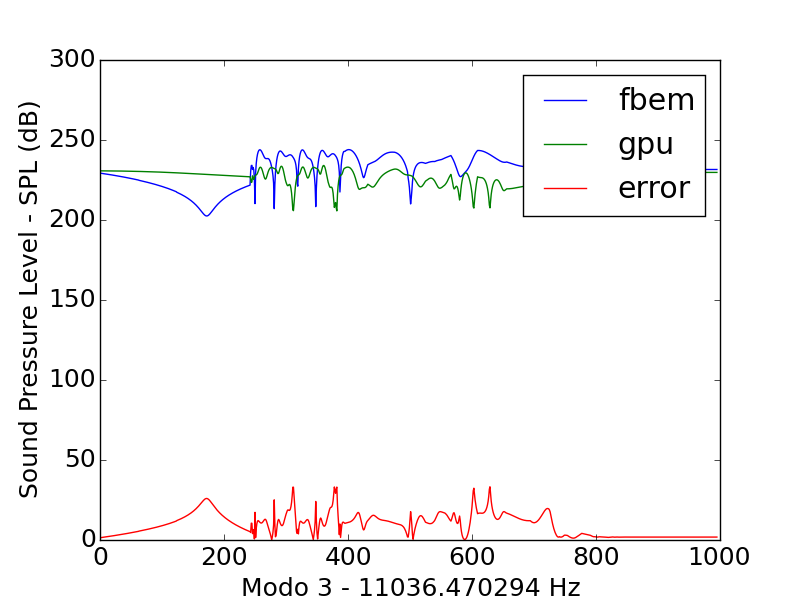
\includegraphics[width=\textwidth]{../data/transfer_test/steel_key/plots/steel_key-tfv-0_3.png}
	\caption{}
	\label{fig:coef_key_3}
\end{subfigure}
\caption[Comparação numérica para a Chave de Aço]{Comparação numérica para a Chave de Aço. A figura ao topo apresenta a diferença numérica média por frequência. As demais figuras apresentam a comparação do módulo dos coeficientes para modos de vibração específicos.}
\label{fig:coef_key_diff}
\end{figure}